\documentclass[border=3pt]{standalone}
% Preâmbulo compartilhado pelos diagramas TikZ da aula 11 (Localização por Grade e Monte Carlo)
\usepackage[T1]{fontenc}
\usepackage[utf8]{inputenc}
\usepackage{lmodern}
\usepackage{amsmath}
\usepackage{xcolor}
\usepackage{tikz}
\usetikzlibrary{arrows.meta,angles,quotes,decorations.pathmorphing,calc,
                positioning,shapes.geometric,shapes.misc,backgrounds,fit,
                math}

% Paleta (mesma dos SVGs originais)
\definecolor{dblue}{HTML}{2A5B8C}
\definecolor{dorange}{HTML}{B3541E}
\definecolor{dgreen}{HTML}{4A7C59}
\definecolor{dred}{HTML}{9C4B4B}
\definecolor{dcream}{HTML}{F4F1EA}
\definecolor{dshade}{HTML}{DDD7C9}

% Função gaussiana (não normalizada por padrão de escala visual)
\pgfmathdeclarefunction{gauss}{3}{%
  \pgfmathparse{1/(#3*sqrt(2*pi))*exp(-((#1-#2)^2)/(2*#3^2))}%
}

% Estilos comuns (prefixo d... para não colidir com chaves internas do pgf)
\tikzset{
  >={Stealth[length=2mm]},
  dguide/.style={gray!55, dashed, line width=0.4pt},
  daxis/.style={gray!60, line width=0.7pt, ->},
  dbody/.style={fill=black!3, draw=black!80, line width=1pt},
  dacc/.style={draw=dblue, line width=1pt},
  dlbl/.style={black!55, font=\small},
  dsub/.style={black!45, font=\footnotesize},
  dstate/.style={circle, draw=black!80, fill=dcream, line width=1pt,
                 minimum size=17mm, font=\large, inner sep=1pt},
  dobs/.style={circle, draw=black!80, fill=dshade, line width=1pt,
               minimum size=14mm, font=\large, inner sep=1pt},
  dbox/.style={rounded corners=2pt, draw=black!80, fill=dcream, line width=1pt,
               align=center, inner sep=6pt},
  dop/.style={circle, draw=black!80, fill=white, line width=1pt,
              minimum size=6mm, inner sep=0pt, font=\small},
  dtrans/.style={->, dblue, line width=1pt},
  dmeas/.style={->, dorange, line width=1pt},
  dcurve/.style={line width=1pt, dblue},
  dcurveb/.style={line width=1.4pt, dorange},
}

\begin{document}
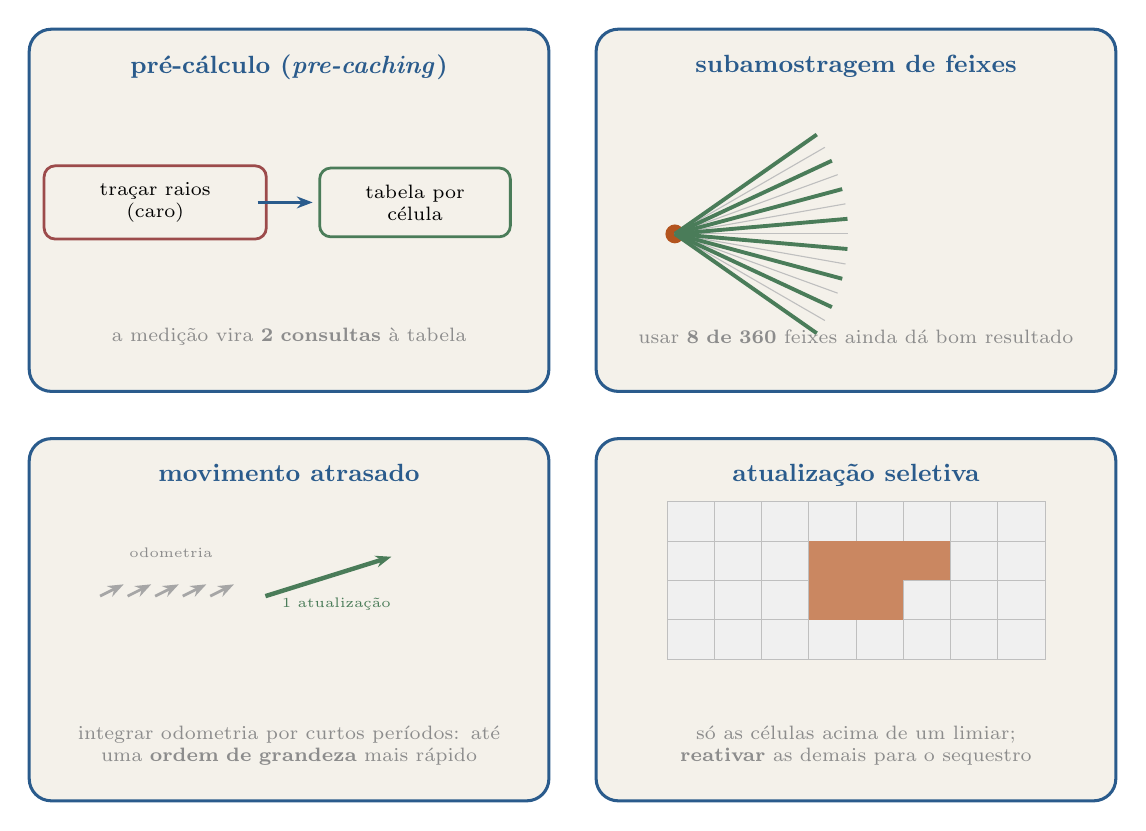
\begin{tikzpicture}[x=1cm,y=1cm,
   cx/.style={dbox, rounded corners=8pt, minimum width=6.6cm, minimum height=4.6cm, draw=dblue, line width=1.1pt, inner sep=0pt}]
  \foreach \x/\y/\t in {0/0/{pré-cálculo (\textit{pre-caching})}, 7.2/0/{subamostragem de feixes}, 0/-5.2/{movimento atrasado}, 7.2/-5.2/{atualização seletiva}} {
    \node[cx] at (\x+3.3,\y+2.3) {}; \node[font=\small\bfseries, dblue, anchor=north] at (\x+3.3,\y+4.4) {\t};
  }
  % 1: pré-cálculo
  \begin{scope}[shift={(0,0)}]
    \node[dbox, rounded corners=4pt, font=\scriptsize, text width=2.4cm, draw=dred] at (1.6,2.4) {traçar raios\\ (caro)};
    \draw[->, dblue, line width=1pt] (2.9,2.4) -- (3.6,2.4);
    \node[dbox, rounded corners=4pt, font=\scriptsize, text width=2.0cm, draw=dgreen] at (4.9,2.4) {tabela por célula};
    \node[dsub, font=\scriptsize, align=center, text width=6cm] at (3.3,0.7) {a medição vira \textbf{2 consultas} à tabela};
  \end{scope}
  % 2: subamostragem
  \begin{scope}[shift={(7.2,0)}]
    \fill[dorange] (1.0,2.0) circle (0.12);
    \foreach \a in {-35,-30,...,35} { \draw[black!25, line width=0.4pt] (1.0,2.0) -- ++(\a:2.2); }
    \foreach \a in {-35,-25,-15,-5,5,15,25,35} { \draw[dgreen, line width=1.4pt] (1.0,2.0) -- ++(\a:2.2); }
    \node[dsub, font=\scriptsize, align=center, text width=6cm] at (3.3,0.7) {usar \textbf{8 de 360} feixes ainda dá bom resultado};
  \end{scope}
  % 3: movimento atrasado
  \begin{scope}[shift={(0,-5.2)}]
    \foreach \i in {0,...,4} { \draw[->, black!35, line width=1pt] ({0.9+\i*0.35},2.6) -- ++(0.3,0.15); }
    \node[dsub, font=\tiny] at (1.8,3.15) {odometria};
    \draw[->, dgreen, line width=1.6pt] (3.0,2.6) -- (4.6,3.1);
    \node[dgreen, font=\tiny, align=center] at (3.9,2.5) {1 atualização};
    \node[dsub, font=\scriptsize, align=center, text width=6cm] at (3.3,0.7) {integrar odometria por curtos períodos: até uma \textbf{ordem de grandeza} mais rápido};
  \end{scope}
  % 4: seletiva
  \begin{scope}[shift={(7.2,-5.2)}]
    \foreach \i in {0,...,7} { \foreach \j in {0,...,3} { \fill[black!6, draw=black!25, line width=0.3pt] ({0.9+\i*0.6},{1.8+\j*0.5}) rectangle ++(0.6,0.5); } }
    \foreach \i/\j in {3/1,4/1,3/2,4/2,5/2} { \fill[dorange!70] ({0.9+\i*0.6},{1.8+\j*0.5}) rectangle ++(0.6,0.5); }
    \node[dsub, font=\scriptsize, align=center, text width=6cm] at (3.3,0.7) {só as células acima de um limiar; \textbf{reativar} as demais para o sequestro};
  \end{scope}
\end{tikzpicture}
\end{document}
